% Masterthesis
%
% Multiscale Modelling Group of Jun.-Prof. Birgit Strodel
%
% Author:
% Oliver Schillinger


\ifdefined\isdraft
    \documentclass[english, a4paper, 12pt, titlepage, draft]{article}
\else
    \documentclass[english, a4paper, 12pt, titlepage, final]{article}
\fi

\usepackage{geometry}
\usepackage[british]{babel}
\usepackage{graphicx,hyperref,url,color,cite}
\usepackage{amsmath}
\usepackage[latin1]{inputenc}

\usepackage{setspace}
\usepackage[version=3]{mhchem}

\hypersetup{
    %bookmarks=false,                      % show bookmarks bar?
    unicode=true,                          % non-Latin characters in Acrobat’s bookmarks
    pdftoolbar=true,                       % show Acrobat’s toolbar?
    pdfmenubar=true,                       % show Acrobat’s menu?
    pdffitwindow=false,                    % window fit to page when opened
    pdfstartview={FitH},                   % fits the width of the page to the window
    pdftitle={Masterthesis},               % title
    pdfauthor={Oliver Schillinger},
    pdfsubject={Masterthesis},             % subject of the document
    pdfcreator={Oliver Schillinger},       % creator of the document
    pdfproducer={Oliver Schillinger},      % producer of the document
    pdfkeywords={Lipase} {CitA} {GROMACS}, % list of keywords
    pdfnewwindow=true,                     % links in new window
    colorlinks=true,                       % false: boxed links; true: colored links
    linkcolor=black,                       % color of internal links
    citecolor=blue,                        % color of links to bibliography
    filecolor=red,                         % color of file links
    urlcolor=cyan                          % color of external links
}


% Figure template
%\begin{figure}
%    \centering
%    
\includegraphics[width=0.5\textwidth]{figures/draft/draft.pdf}
%    \caption{}
%    \label{fig:}
%\end{figure} 


% ============================================================================ %


\begin{document}

% ============================================================================ %

\begin{titlepage}
\begin{center}
{\huge \textbf{Masterthesis}}\\
\vspace{2cm}
{\large \textbf{Protein Structure and Dynamics} \\
\vspace{1cm}
of \textit{Bacillus Subtilis} Lipase LipA Fused to the Ligand-Binding Domain of Sensor Histidine Kinase CitA
}

\vspace{2cm}

Oliver Schillinger \\
Forschungszentrum J\"ulich \\ Institute of Complex Systems 6 - Structural Biochemistry \\ Multiscale Modelling Group \\
Supervisor: Jun.-Prof. Dr. Birgit Strodel \\
\vspace{1cm}
German Research School for Simulation Sciences \\
RWTH Aachen

\vspace{1cm}

\today

\vfill

\begin{figure}[h!]

\includegraphics[width=.3\textwidth]{figures/logos/grs_logo.pdf}
\hspace{0.5cm}

\includegraphics[width=.3\textwidth]{figures/logos/fzj_logo.pdf}
\hspace{0.5cm}

\includegraphics[width=.3\textwidth]{figures/logos/rwth_logo.pdf}
\end{figure}
 
\end{center}
\end{titlepage}


% ============================================================================ %

\onehalfspacing

\begin{abstract}

The structure and kinetics of two proteins under investigation are well known:
The periplasmic domain of sensor \textit{Klebsiella pneumoniae} histidine kinase CitA (PDB accession code \href{http://pdb.rcsb.org/pdb/explore/explore.do?structureId=2J80}{2J80}) \cite{CitA_2J80}
and the lipase LipA of \textit{Bacillus subtilis} (BSLA, PDB accession code \href{http://pdb.rcsb.org/pdb/explore/explore.do?structureId=1I6W}{1I6W}), \cite{BSLA_1I6W} both in their ligand bound and ligand free states.
What is not understood is the structure and kinetics of a fusion protein of these two peptides.
Experiments indicate that citrate binding to the kinase down-regulates lipase activity (Figure \ref{fig:BSLAactivity}).
This effect is of major interest to the chemical industry as lipases exhibit a wide diversity in substrate specificity and have found applications in the resolution of racemic mixtures, the synthesis of esters, transesterification reactions and as additives in laundry detergents.
As chemical applications would benefit from the opposite effect, a controlled up-regulation of lipase activity triggered by citrate addition, this research focused on the structure elucidation of the fused protein, as well as on the mechanism by which lipase activity is regulated.
A thorough understanding of this mechanism might in the future enable us to engineer the protein to invert the regulatory effect of citrate binding.
The main methods used for structure elucidation are global optimization using the Monte Carlo-minimization approach basin hopping, followed by high-throughput molecular dynamics simulations. 

\end{abstract}


% ============================================================================ %

\tableofcontents

\pagebreak

\onehalfspacing

% ============================================================================ %

\section{Introduction}

\begin{figure}
    \centering
    
\includegraphics[width=0.5\textwidth]{figures/draft/draft.pdf}
    \caption{The activity of the BSLA -- CitA complex is reduced after citrate addition while the uncomplexed lipase is not affected. Experiments performed by Karl Erich Jaeger et al., data unpublished.}
    \label{fig:BSLAactivity}
\end{figure}


% ============================================================================ %

\section{Proteins Under Investigation}

% ==================================== %

\subsection{\textit{Bacillus Subtilis} Lipase LipA}

\textit{Bacillus Subtilis} is a gram-positive, aerobic bacterium found in soil and water that is subject to active research since 1992 \cite{bacillusSubtilis}.
\textit{Bacillus Subtilis} is of major industrial interest because of its highly efficient protein secretion system \cite{BSsecretion} enabling the production of proteases and amylases in bulk quantities \cite{BSworkhorse}.
Of special interest are its excreted lipases as these catalyze the hydrolysis and synthesis of long chain triacylglycerols \cite{BSLA_1I6W}.
These lipases possess a wide substrate specificity.
They find applications in transesterification reactions, the synthesis of esthers, the resolution of racemic mixtures and are used as additives in laundry detergents \cite{BSdetergents}.

In the reported experiments lipase LipA from \textit{Bacillus Subtilis} was used (hereafter called BSLA).
Compared to lipases from other organisms its size is relatively small, consisting of 181 amino acids and weighting slightly more than 19 kDA.
BSLA belongs to the $\alpha$-$\beta$ hydrolase fold enzymes.
This protein family are constituted by a twisted $\beta$-strand core flanked by alpha helices on both sides \cite{alphaBetaHydrolases}.
Because of its small size it can be considered a minimal $\alpha$-$\beta$ hydrolase.
BSLA hydrolyses sn-1 and sn-3 glycerol esthers with long fatty acid chains, while its highest activity is exhibited on medium sized fatty acids \cite{BSLA_1I6W}.
The optimum activity is reported to be found at pH 10 \cite{BSLA_1I6W}.
Most known lipases possess an $\alpha$-helical segment that covers the active site.
The encounter of lipid-aggregates triggers the opening of this lid, exposing the active site and triggering catalytic activity.
This behaviour is known as interfacial activation \cite{alphaBetaHydrolases}.
This lid is absent in BSLA.

BSLA lacks this lid, resulting in an active site that is solvent exposed.
The active site is located at the bottom of a shallow cleft formed by four turns (Figure \ref{fig:BSLAactiveSite}).
Its structure is in accordance with the secondary structure topology of the canonical $\alpha$/$\beta$-hydrolase fold, in which the acitve site is formed by a nucleophile, an acid and a histidine, called the catalytic triad \cite{BSLA_1I6W}.
This catalytic triad is constituted of Ser77 (nucleophile), Asp133 (acid) and His156.
Serine 77 is located at the so called nucleophilic elbow \cite{nucleophileElbow}, a sharp turn at the bottom of the binding pocket.
The ester hydrolysis catalyzed by BSLA is depicted in Figure \ref{fig:BSLAreaction}.
The ligand binds covalently with its phosphonyl group to Ser77.
A tetrahedral intermediate structure is formed.
One phosphonyl oxygen of the substrate is hydrogen bound to the \ce{NH} atoms of Met78 and Ile12, forming the oxyanion hole that is common to most lipases \cite{BSLA_1I6W}.
The \ce{N^{$\epsilon$}} atom of His156 is located at hydrogen bonding distance from the Ser77 \ce{O^{$\gamma$}} atom and the substrate esther oxygen.






\begin{figure}
    \centering
    
\includegraphics[width=0.5\textwidth]{figures/draft/draft.pdf}
    \caption{Active site of \textit{Bacillus Subtilis} lipase LipA.}
    \label{fig:BSLAactiveSite}
\end{figure} 

\begin{figure}
    \centering
    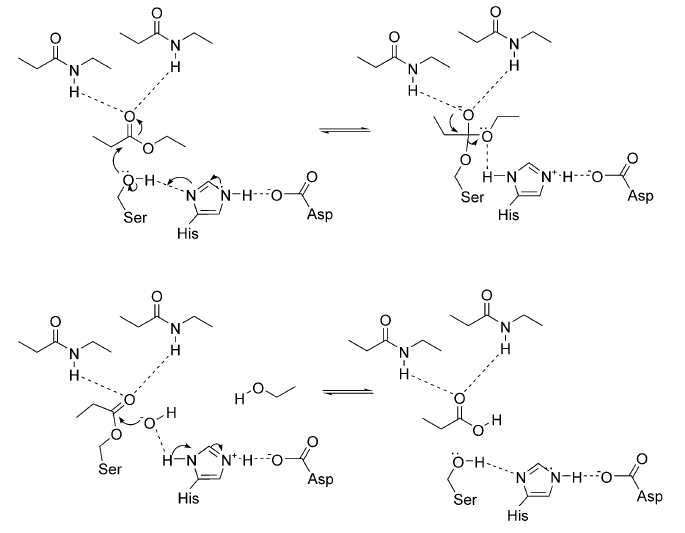
\includegraphics[width=0.7\textwidth]{figures/BSLA_reaction.png}
    \caption{Ester hydrolysis reaction catalyzed by BSLA. Taken from \cite{BSLA_reaction}.}
    \label{fig:BSLAreaction}
\end{figure}  





% ==================================== %

\subsection{Periplasmic Domain of Sensor Histidine Kinase CitA}

% ==================================== %

\subsection{Fusion Complex}


% ============================================================================ %

\section{Methods}
\subsection{Molecular Dynamics}
\subsubsection{Force Fields}
\subsubsection{Water Model}
\subsection{Basin Hopping with GMIN}
\subsection{pKa Prediction}
\subsection{k-Means Clustering}


% ============================================================================ %

\section{Simulation Setups}
\subsection{Equilibration}
\subsection{Production Runs}


% ============================================================================ %

\section{Results}


% ============================================================================ %

\section{Discussion \& Conclusion}


% ============================================================================ %

\section{Outlook}
The results should be combined with experimental data from small angle X-ray scattering, and NMR experiments. The mechanism of activity regulation is investigated with the help of non-equilibrium molecular dynamics.


% ============================================================================ %

\section{Acknowledgments}


% ============================================================================ %

\singlespacing
\small

\bibliographystyle{unsrt}
\bibliography{masterthesis}
 
% ============================================================================ %

\end{document}
 
